\documentclass{article}

% required 
\usepackage[hyphens]{url} % this wraps my URL versus letting it spill across the page, a bad habit LaTeX has
\usepackage{Sweave}
\usepackage{graphicx}
\usepackage{natbib}
\usepackage{amsmath}
\usepackage{textcomp}%among other things, it allows degrees C to be added
\usepackage{float}
\usepackage[utf8]{inputenc} % allow funny letters in citations 
\usepackage[nottoc]{tocbibind} %should add Re fences to the table of contents?
\usepackage{amsmath} % making nice equations 
\usepackage{listings} % add in stan code
\usepackage{xcolor}
\usepackage{capt-of}%allows me to set a caption for code in appendix 
\usepackage[export]{adjustbox} % adding a box around a map
\usepackage{lineno}
\linenumbers
% recommended! Uncomment the below line and change the path for your computer!
% \SweaveOpts{prefix.string=/Users/Lizzie/Documents/git/teaching/demoSweave/Fig.s/demoFig, eps=FALSE} 
%put your Fig.s in one place! Also, note that here 'Fig.s' is the folder and 'demoFig' is what each 
% Fig. produced will be titled plus its number or label (e.g., demoFig-nqpbetter.pdf')
% make your captioning look better
\usepackage[small]{caption}

\usepackage{xr-hyper} %refer to Fig.s in another document
\usepackage{hyperref}

\setlength{\captionmargin}{30pt}
\setlength{\abovecaptionskip}{0pt}
\setlength{\belowcaptionskip}{10pt}

% optional: muck with spacing
\topmargin -1.5cm        
\oddsidemargin 0.5cm   
\evensidemargin 0.5cm  % same as odd side margin but for left-hand pages
\textwidth 15.59cm
\textheight 21.94cm 
% \renewcommand{\baselinestretch}{1.5} % 1.5 lines between lines
\parindent 0pt		  % sets leading space for paragraphs
% optional: cute, fancy headers
\usepackage{fancyhdr}
\pagestyle{fancy}
%\fancyhead[LO]{Frederik Baumgarten}
%\fancyhead[RO]{Research Proposal}
% more optionals! %
\usepackage{booktabs} %clean and professional look for tables

\graphicspath{ {/Users/frederik/github/PhaenoFlex_clean/docs/figs/} }% tell latex where to find figures 

\begin{document}
%	\renewcommand{\bibname}{References}%names reference list 
	
	
	%	\title{
		%	} 
	
	
	\date{\today}
	
	\section*{Aim}
	As climate continues to warm, ecosystems are facing more extreme heat and drought waves. At the same time the potential growing season of temperate and boreal latitudes extends. To which degree plants and forests adapt and indeed prolong their photosynthetic activity in spring and autumn is currently under heavy debate. Not only may soil moisture resources limit plant activity and overall performance but also internal growth control mechanisms could limit further Carbon uptake from the atmosphere. Therefore, this experimental study aimed to provide evidence how longer climatic growing seasons translate into increased biomass production in relation to the negative impacts of drought and heat events. 
	
	\section*{Methods}
	\subsection*{Study species and study site}
	3 year-old saplings of 6 species, each representing a different family were selected to get a wide range of possible tree responses including coniferous evergreen and broad leaved deciduous species. All species selected occur naturally along the Pacific west coast of USA and Canada. The studied deciduous trees were \textit{Prunus virginiana} L., \textit{Acer macrophyllum} Pursh., \textit{Betula papyfera} Marsh. and \textit{Quercus garryana} Dougl.; evergreen trees were \textit{Pinus contorta} Dougl., and \textit{Sequoia sempervirens} (D. Don) Endl. In the following we refer to their genus name only.
	
			\begin{table}[H]
		\centering
		\caption{Species information}
		\begin{tabular}{p{5.8cm} p{2cm} p{2.0cm} p{1.0cm} p{3cm}}
			\toprule
			\textbf{Species name} & \textbf{Family} & \textbf{Initial height} & \textbf{drought tolerance} & \textbf{remarks} \\
			\midrule
			\textit{Prunus virginiana L.} & Rosaceae & x & x &  x  \\
			\textit{Acer macrophyllum Pursh.} & Sapindaceae & x & x & x \\
			\textit{Betula papyfera Marsh.} & Betulaceae &x & x & x \\
			\textit{Quercus garryana Dougl.} & Fagaceae & x & x & x \\
			\textit{Pinus contorta Dougl.} & Pinaceae & x & x &  x\\
			\textit{Sequoia sempervirens (D. Don) Endl.} & Cupressaceae & x & x & x \\
			
			\bottomrule
		\end{tabular}
	\end{table}
	
	
	%	\begin{table}[h!]
	%	\begin{center}
		%	\caption{Details of saplings origin }
		%	\label{tab:table1}
		%	\begin{tabular}{l|c|r} % 
			%	\textbf{Species} & \textbf{Nursery} & \textbf{Seed origin}\\
				%$\alpha$ & $\beta$ & $\gamma$ \\
			%	\hline
			%	Prunus virginiana L. & Peel's Nurseries Ltd. & BC Canada\\
			%	Acer macrophyllum Pursh. & Streamside Native Plants & BC Canada\\
			%	Betula papyfera Marsh. & Peel's Nurseries Ltd. &BC Canadac\\
			%	Quercus garryana ?.& Peel's Nurseries Ltd. & BC Canada\\
			%	Populus trichocarpa Torr. & Peel's Nurseries Ltd.& BC Canada\\
			%	Pinus contorta, Dougl. & Tree Time Services Inc & Alberta Canada\\
			%	Sequoia sempervirens(D. Don)&? & California\\
				
			%\end{tabular}
		%\end{center}
	%\end{table}
	
	
	The study was conducted on the campus of the University of British Columbia (Totem Field; 49.2572 N, -123.2503 E) located in Vancouver, Canada. The climate is oceanic characterized by the proximity of the Pacific with a mean annual temperature around 10°C (18°C in July and 4°C in January). Together with an annual precipitation of c. 1500mm this climate supports a typical temperate rain forest along the west coast. %Vancouver has been subjected to heat waves in the past years. For instance, the greater Vancouver area has been strucked with severe heat waves in 2009 and 2021 that lasted extended periods (Henderson et al., 2016; Henderson, McLean, Lee, Kosatsky, 2022). In addition of those very rare temperature, 2021 heat dome was characterised by near peak daylight hours and high night temperature (Henderson et al., 2022). 
	
	\subsection*{Experimental setup}
		
	Saplings arrived in Winter 2023 and were, still dormant, repotted using a medium for perennials consisting of 50\% peat, 25\% crushed pumice and 25\% crushed bark (www.westcreekfarm.com). The low water-retention capacity of this potting medium allowed to accelerate and intensify the effects of the drought treatments. Soil volume was adjusted for each species, specifically doubled in volume compared to the previous container to minimize limitations later in the season (final pot volume: 4.5l for Sequoia and Pinus; 9l for Quercus and Betula; 18l for Acer and Prunus). \\ 
	After potting, saplings received 2g of slow-release NPK fertilizer (osmocote plus) to meet natural conditions. \\ 
	On 31 March 2023, saplings were transferred to cooling chambers set at 4°C with ambient photoperiod conditions to prolong dormancy for one month (until 30 April 2023). The only exception was the saplings designated for growing season extension, which remained at the experimental site. \\ 
	Saplings were then arranged in three blocks, each containing a subset of all treatments. Two blocks were sheltered from rain by an open-walled and well ventilated polytunnel greenhouse to protect sensitive electronics. All saplings were attached to a drip irrigation system (40 PVC frame from Netafilm with a Toro controler) that ensured saturated soil moisture conditions throughout the experiment (120±6 ml water every 6 hours;  except for the drought treatment duration). \\ 
	
		\subsection*{Study design and treatments}
	The whole study design is depicted in Fig. \ref{fig:fig_1xxx} for an overview. Saplings were subjected to a) a growing season extension, b) one out of 3 drought timings, c) one out of 3 defoliation events and d) a heat event, resulting in eight treatments plus control. 15 replicates were randomly assigned to each treatment (8 treatments plus control à 15 replicates = 135 saplings/species). \\  
	
			\begin{figure}[H]
		\centering
		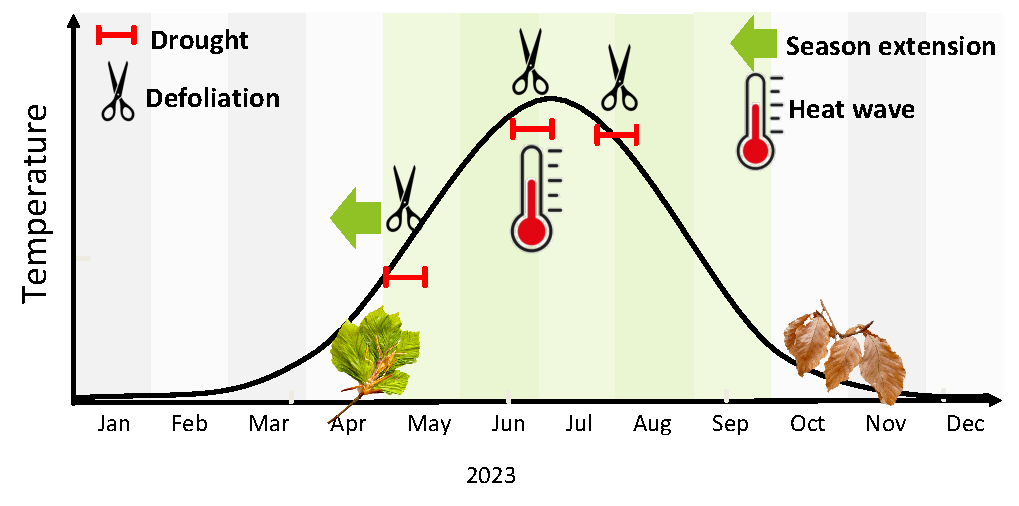
\includegraphics[width=0.9\textwidth]{design_schematic.pdf} 
		\caption{Schematic overview of the average temperature curve at the field site with the vegetation season in green. Depicted are all types and timings of treatments during the year 2023 }
		\label{fig:fig_1xx}
	\end{figure}
	
	\textit{Growing season extension} \\
	Growing season extensions were achieved by prolonging dormancy of all other treatments for a month (see above). Hence sampling of this treatment accumulated xxx more growing degree days (GDD) by being exposed to ambient conditions. Depending on species this `warming' advanced budburst by X to Y days (see XX).\\
	
	\textit{Drought treatments} \\
	Drought treatments were conducted in climate chambers (TPC-19, Biochambers; Canada) at close proximity to the experimental site (Faculty of Forestry, UBC). Drought conditions were simulated with temperatures set to 30°C during the day and 20°C at night. These temperatures rose and fell at the same time every day, corresponding to the photoperiod at Vancouver’s summer solstice (i.e. photoperiod: 16h and 15min). The photoperiod was adjusted weekly, to the current ambient sunrise and sunset time. 
	The first drought treatment started species-specific once leaf-out reached stage 4 (i.e. leaves fully unfolded). Second and third drought treatment were started on a fixed date, namely 23 June and 31 July 2023. Subsequent drying of the pots was monitored by measuring whole pot weight (balance accuracy 0.1g) as well as volumetric water content (VWC, Fieldscout TDR 150). Saplings were released from drought stress on species-specific dates, marked by the first signs of desiccation, such as curled or discolored leaves, and soil moisture levels approaching the wilting point. %for several days...curves? or even argue with poor recovery during the night of stem diameter 
	Saplings were again weighted under field capacity and then transferred back to the experimental site and plugged into the irrigation system. \\
	
	%For the first drought treatment dehumidifiers (Toshiba TDDP2213ES2) were set in the climate chambers at a set humidity of 35%, in order to avoid relative humidity differences that could affect the tree’s transpiration rate
	
	\textit{Defoliation treatments} \\
	The defoliation treatments were intended to simulate leaf loss due to frost, browsing, hail or overheating. As these scenarios cause different physiological reactions (e.g. release of defence substances), we cut off each fully unfolded leaf (stage 4) halfway up the petiole using pruning scissors. Younger stages were left intact to prevent accidental damage to the meristem. The leaf area was reduced to 0\% for all deciduous species. For pines, all needles older than 1 year were removed by hand by tearing them delicately in the direction of the apex. The current year needles were preserved in the first defoliation treatment since they were less than 1cm in length and still developing. In the second and third defoliation event c. ¾ of the current-year needles were removed, which presumably contributed already most to the total photosynthetic assimilation. All defoliation events coincided with the start of the respective drought treatments, i.e. the first defoliation took place on the same day as the start of the first drought treatment. In the following two weeks we continuously cut all newly emerging leaves reaching stage 4 to suspend all assimilate supply. %mention here the weight of the leaves	All the leaves collected were gathered in brown paper bags, where all the replicates from the same species were put together to dry. The leaves were dried for 48 hours at 70°C in a drying oven (VWR 1645D). Dry matter biomass was measured with scale (Scout Pro) to an accuracy of two decimal places (0.00 grams).
	Subsequent recovery of saplings was assessed by eye as the percentage of recovering leaf area compared to a control sapling. Sequoia saplings were not included in this treatment.\\
	
	\textit{Heat treatment} \\
	The simulated heat wave (walk in climate chamber, LTRB, BioChambers) aimed to bring saplings to their upper temperature threshold where growth and photosynthesis ceases. The treatment started together with the second drought timing (23 June) and lasted the same species-specific duration. Temperature followed ambient photoperiod with temperature reaching up to 39°C during the day and 29°C during the night. Saplings were watered every day to saturation and relative humidity was around 90\% to avoid cooling by transpiration. 
	

	
	\subsection*{Phenological monitoring}
		\textit{Leaf emergence} \\
	Bud development in spring was assessed by the same observer twice a week starting 24 April 2023 using a categorical scale depending on species. Deciduous species were scored on a four-stage scale (see \citep{vitasseElevationalAdaptationPlasticity2013a}): stage 0 - dormant, stage 1 - bud swelling, stage 2 - bud burst, stage 3 - leaf-out and stage 4 - leaf unfolded. Pine saplings were scored differently as follows: stage 1 - swelling or elongation of shoot visible, stage 2 - green needle tips along the shoot visible, stage 3 - scales open along the shoot and first needles become visible, stage 4 - green needles emerging away from the shoot. Phenostages for Sequoia were limited to two stages because this species does not form buds: stage 1 - first signs of needles visible at the apical meristem but all bended inwards towards the center, stage 2 - needles start to grow and bend outwards from the center.
	For all species and saplings the day of year was recorded as soon as 50\% of all buds reached the newest stage. \\
	
		\textit{Bud set} \\
		Cessation of bud development was monitored starting in early July 2023 until the apical bud was dormant. Bud set was generally scored on a four-stage score as follows: stage 3 - ongoing shoot growth/elongation, stage 2 - apical bud forms and remains as a light-green bud with the last (pair) of leaves remaining small, stage 1 - first bud scales appear, stage 0 - bud turns dark red/brown and hardens. In Acer only stages 3, 2 and 0 were distinguished and recorded. Bud set of Pinus and Sequoia were not monitored, since shoot elongation was the best activity proxy of the shoot apical meristem.\\
		
		\textit{Leaf senescence} \\
		Leaf senescence was monitored in weekly intervals between 1 Sept 2023 and 4 Nov 2023 i.e. until all leaves were shed. For each sapling and at every monitoring occasion the chlorophyll content was estimated using a leaf spectral index (LSI; mean of three representative leaves per replicate; MC-100, apogee instruments). Following  \citep{zohner} this value was weighted by simultaneous estimates of the percentage of remaining green leaves (by eye; 100\%=all leaves remaining; 0\%=all leaves shed). For example, a sapling with 50\% remaining leaves and a mean LSI of 10 was rated with a total LSI of 10 (0.5 * 20). A sapling was considered senescent one a value was below 50\% of the maximum LSI value. \\
		%In addition, light curves, Amax measurements
		
		
		
			
\begin{table}[H]
	\captionsetup{justification=raggedright, singlelinecheck=false} % Left-align caption
	\centering
	\caption{Phenological stages used for all deciduous species \citep{vitasseElevationalAdaptationPlasticity2013a}, pine as well as Sequoia}
	\begin{tabular}{p{2.4cm} p{1cm} p{2.5cm} p{8.0cm}} % Make sure the formatting is correct
		\toprule
		\textbf{Group} & \textbf{Scale} & \textbf{Phenostage} & \textbf{Description} \\
		\midrule
		
		\multicolumn{4}{l}{\textit{Deciduous species}} \\
		& 0 & dormant & no bud development visible \\
		& 1 & bud swelling & swollen and/or elongating buds \\
		& 2 & budburst & bud scales open and leaves partially visible \\
		& 3 & leaf-out & leaves fully emerged from bud but still folded, crinkled or pendant \\
		& 4 & leaf unfolding & leaves fully unfolded \\
		\midrule
		
		\multicolumn{4}{l}{\textit{Pine}} \\
		& 0 & dormant & no signs of activity \\
		& 1 & swelling & swelling or elongation of shoot visible \\
		& 2 & budburst & green needle tips along the shoot visible \\
		& 3 & leaf-out & scales open along the shoot and first needles become visible \\
		& 4 & leaf-unfolding & green needles emerging away from the shoot \\
		\midrule
		
		\multicolumn{4}{l}{\textit{Sequoia}} \\
		& 1 & not active & first signs of needles visible at the apical meristem but all bent inwards towards the center \\
		& 2 & active & needles start to grow and bend outwards from the center \\
		\bottomrule
	\end{tabular}
\end{table}


			
	\subsection*{Soil moisture measurements}
Soil drying during drought treatments was documented with daily volumetric water content (VWC) measurements using a soil moisture meter (Fieldscout TDR 150; rod length 12cm or 20cm for small or large pots, respectively). In addition, and for a more integrated indicator of soil water loss near the wilting point, whole pots were weighted using a scale (accuracy ±1g). Replicates equipped with magnetic dendrometers were weighted at the start and end of the drought treatments only.  %Since VWC and weight loss yielded a strong correlation (Fig SX) whole VWC curves were calculated also for these replicates.\\

	\subsection*{Shoot apical growth}
	Shoot growth activity of the apical meristem was measured on 10 replicates per treatment throughout the season in biweekly intervals. Water resistant measuring tapes were attached to the stem base under the terminal bud after budburst and subsequent shoot elongation was tracked on the tape.  \\

	\subsection*{Radial growth and tree-water deficit}
To track radial growth, magnetic dendrometers were installed that were designed to not injure the bark during installation and operate without friction \citep{clonchHighPrecisionZerofriction2021}. Devices were installed at the stem base avoiding branches and abnormalities using breathable bandage material (). Five control replicates were equipped permanently while drought treatments swiched devices so that five replicates of every drought timing captured diameter fluctuations 1 week prior, during and 2 weeks after the respective drought treatment. \\ % mention Swiss dendrometers to check reliability and accuracy

	\subsection*{Biomass assessment}
	Before budburst and after the growing season we measured diameter c. 2 cm above plant collar (digital calliper; accuracy ±0.1mm) and height (graduated pole; accuracy ±1mm) of each sapling. Total above-ground biomass was estimated following allometric equations provided by \citet{annighoferSpeciesspecificGenericBiomass2016}. Substracting before from after season estimates revealed the calculated above-ground biomass increment.	\\
After entering full dormancy, all saplings were removed from pots in December 2023 to wash off the potting substrate. Whole saplings where dried at 80° C for 48h before tissue was separated into roots and shoots with the latter being further sorted into current year and past years tissue. All partial quantities were weighted to an accuracy of ±0.01g.\\ %Scout Pro

	\subsection*{Wood anatomy}
Prior to every drought and defoliation event, 10 replicates were pinned at a homogenous stem section at the base using a needle and dyed with ethylene blue \citep{gartnerCambialActivityMoringa2021a}. This pinning hole acted as a `marker in time' that allowed to separate wood formation before and after treatment start. During harvest at the end of the growing season, a 2cm section containing the pinning hole was cut using an electric saw and stored in 35\% ethanol solution. \\
C. four stem sections per replicate were cut using a microtome (semi-automated Lab-microtome, WSL; thickness: 15\textmu m) to ensure the visiblilty of the anatomical structure around the pinning hole. Sections were double stained with Safranin (to color lignified structures red) and Astrablue (to color unlignified structures blue) following standard protocol \citep{gartnerMicroscopicPreparationTechniques2013}. Sampled where then fixed using UV-sensitive mounting medium (Eukitt UV, Fisher scientific) and dried under a commercial nail dryer UV-lamp for c. two minutes. Samples where then scanned with a slide scanner () and then processed with xxxx.

	\subsection*{Data analysis and statistics}
	
	
				\newpage
				
	\section*{Preliminary results}
	The experiment was conducted with minor adjustments to the proposed project. While data processing is still ongoing with two manuscripts in preparation we present here first insights.
	
	\subsection*{Apical shoot growth}
	Shoot elongation showed species-specific patterns with distinct determinate to indeterminate behaviour. Acer, Prunus and Quercus ceased apical shoot growth shortly after preformed tissue in buds was elongated (few weeks after budburst; see Fig. \ref{fig:shoot_elongation copy}). In contrast Betula, Sequoia and to some extent Pinus showed continues growth throughout the season, in some cases until low temperature in autumn induced senescence of the foliage.
	
				\begin{figure}[H]
		\centering
		\includegraphics[width=0.9\textwidth]{shoot_elongation copy.pdf} 
		\caption{Shoot extension over the growing season 2023 for the six study species. Note the species-specific differences in absolute growth and in growth phenology with Quercus stopping first and Sequoia elongating until the very end of the season.}
		\label{fig:shoot_elongation copy}
	\end{figure}
	
				\newpage
		\subsection*{Radial cambial growth}
		The specifically designed magnetic dendrometers performed well and yielded very accurate and comparable results compared to standard point dendrometer (see Fig. \ref{fig:dendrometer_graph}). Measurements during and after drought treatments indicated strong tree water deficits with strong stem shrinkage and almost no recovery during the night (Fig. \ref{fig:dendrometer_graph}). Together with soil moisture measurements this is prove of severe drought conditions. Nevertheless most individuals showed strong recovery after drought stress release. 
		
					\begin{figure}[H]
			\centering
			\includegraphics[width=0.9\textwidth]{dendrometer_graph.pdf} 
			\caption{Left: Newly developed magnetic dendrometer (at the stem base) were used to monitor radial growth in a 15 min interval. Their performance was compared to classical point dendrometers (upper part of the stem). Right: Example of the changes in stem diameter of a Bigleaf maple sapling during a drought treatment and subsequent recovery phase.}
			\label{fig:dendrometer_graph}
		\end{figure}
		
			\subsection*{Biomass}
			\textit{Effect of different treatment applied at the same time}\\
			Total biomass at the end of the growing seasons was lowest for saplings of all species that were defoliated --- surprisingly even lower than drought-exposed saplings. Although saplings needed a longer recovery from defoliation than from drought stress, Quercus as a fully recovering species that quickly re-flushes from dormant spare buds, showed most reduced biomass compared to control saplings (Fig. \ref{fig:biomass_post_solst_treat_sub}). Growing season extensions had small and mixed effects with Prunus as the only species showing a significant increase in biomass compared to control saplings. Heating close to a species upper tolerance threshold had surprisingly no negative effects on biomass, despite obvious signs of stress (brownish leaves). On the contrary, Betula and Prunus increased biomass compared to control saplings.
			\\
			
			\textit{Effect of different timings of same treatments}\\
			Comparing different timings of drought and defoliation events revealed that biomass accumulation and therefore growth is mostly sensitive to stress around the summer solstice. However, drought had also little effects on biomass just after leaf-out and was neglictable in August. Defoliation had even a small positive effect on biomass accumulation in Prunus, Betula and Pinus. Presumably these species were able to compensate later in the season as was observed by a later date of senescence (data not shown here).
			\\
			
				
			\begin{figure}[H]
				\centering
				\includegraphics[width=0.9\textwidth]{biomass_post_solst_treat_sub.pdf} 
				\caption{Effect size in g of biomass compared to control sapling when exposed to an extended growing season (GS\_extend), heat, defoliation or drought event. Colors represent the six study species. Shown are means±SD of the posteriors. Prvi: Prunus; Acma: Acer; Quma: Quercus; Bepa: Betula; Pico: Pinus; Sese: Sequioia.}
				\label{fig:biomass_post_solst_treat_sub}
			\end{figure}
			
							\begin{figure}[H]
				\centering
				\includegraphics[width=0.9\textwidth]{biomass_post_treat_sub.pdf} 
				\caption{Effect size in g of biomass compared to control sapling when exposed to defoliation or drought treatments on 3 occasions. Colors represent the six study species. Shown are means±SD of the posteriors. Prvi: Prunus; Acma: Acer; Quma: Quercus; Bepa: Betula; Pico: Pinus; Sese: Sequioia.}
				\label{fig:biomass_post_treat_sub}
			\end{figure}
			
			
				\subsection*{Wood anatomy}
				Data processing is still under way due to the underestimated time required.
				
				\begin{figure}[htbp]
					\centering
					\includegraphics[width=0.9\textwidth]{pinning_overview_2.pdf} 
					\caption{Left: stem section cut with an electrical saw close to the marked pinning hole. Right: 15\textmu m cross-section of \textit{Betula papyrifera} double stained with Astrablue and Safranin. Pinning holes are indicated with the arrow}
					\label{fig:pinning_overview_2}
				\end{figure}
				\begin{figure}[htbp]
					\centering
					\includegraphics[width=0.9\textwidth]{pinning_closup_x2.jpg} 
					\caption{Cross-section of \textit{Quercus garryana} depicting the reaction caused by the pinning. A: pinning hole with bark and phloem cells; B: zone of irritated cambial cells surrounding the pinning hole (callose tissue); C: border of cambium at the time of pinning; D: Pinning hole penetrating into the xylem cells that were already formed at the time of pinning; E: xylem cells formed prior to pinning; F: xylem cells formed after pinning. }
					\label{fig:pinning_closup_x2}
				\end{figure}
				
				
				
		\section*{Conclusions and outline}
			Preliminary results indicate that defoliation has a stronger negative impact on growth than drought or heat and that the induced growing season marginally affected growth performance compared to control saplings. Moreover, effects of stress timing on biomass accumulation matters and is most pronounced in end of June when growth is commonly observed to peak. The pronounced effect of leaf removal, despite fast recovery in most species is surprising because trees are thought to be sink-limited: cell division and maturation are thought to be the most critical and sensitive physiological processes with sugar assimilates often used from reserves. Our data indicate that the formation of new tissue is indeed dependent on fresh assimilates. Moreover, determinate species, that rely on pre-build leaves for the entire season only, appear to be most affected from defoliation events. Indeterminate growing species, in contrast, may compensate stress episodes by prolonging or shifting their growth phenology. Such a phenotypic plasticity may become crucial in a climate with increased frequency of environmental stress and should be further investigated as an important functional trait.\\
			
			Our results also emphasize that the effects of environmental stress may not become apparent in the current year but could rather manifest in the subsequent year. Determinate species, in particular, are likely to experience reduced performance in the following year, as their entire next year's foliage is formed in the current year, eventually under poor conditions. This in turn may largely define the growth potential  in the upcoming year.\\
			
			Depending on how much tissue is pre- versus neo-formed in a current growing season, species may perform differently under environmental stress. This finding has inspired two follow-up projects: 1) a literature search was launched to review the concept of (in)determinism and to screen species for their degree of indeterminism. A conceptual figure is depicted in Fig. \ref{fig:determinismFigure_FB}. 2) an experiment was launched to investigate how warming in spring and/or autumn affects growth performance not only in the current but also in the following year (carry over effect). Part of this work was presented at ESA, Longbeach, CA and EGU, Vienna. 
			
	\begin{figure}[H]
	\centering
	\includegraphics[width=1.1\textwidth]{determinismFigure_FB.pdf} 
	\caption{Determinate and indeterminate growth within one growing season for species producing terminal buds. Commonly all tree species deploy buds during their first (spring) flush from prebuilt and overwintering leaf primordia (A). Determinate growing species set buds (B) that are under hormonal suppression to inhibit any further activity of the shoot apical meristem (paradormancy). Indeterminate growing species continue to produce new tissue directly (C) or through one (D) to several (E) intermediate bud stage(s). Finally, most species set their bud (F) and enter full dormancy (endodormancy). Shoot apical meristem (SAM); Bud scale (BS); leaf primordia (LP). The basic unit of a shoot is the phytomer which is composed of a node, a leaf, the axillary bud and an internode.}
	\label{fig:determinismFigure_FB}
	\end{figure}
	
	
		\begin{figure}[H]
	\centering
	\includegraphics[width=0.9\textwidth]{design.pdf} 
	\caption{Daily mean (solid black line) and min/max (shaded area) temperature as well as photoperiod at the experimental site at UBC. Temperature during the three drought treatments are shown in yellow, orange and red. Arrows indicate defoliation events.}
	\label{fig:design}
\end{figure}
	

	
	

	
	

	
	
	

	
	
	%\section*{stuff I did't find place yet}
	
	
	\newpage
	
	
	\bibliography{refs_phaenoflex}
	\bibliographystyle{ecolett}
	
	
	
	
	
	
\end{document}
